\documentclass{homework}
\usepackage{float}
\usepackage[dvipsnames]{xcolor}
\usepackage{tikz}

\title{Tarea 1}
\date{2019-09-06}
\gdate{2do Semestre 2019}
\author{Nicholas Mc-Donnell}
\course{Variable Compleja - MAT2705}

\begin{document}
\maketitle
\pagenumbering{roman}
\newpage
\tableofcontents
\newpage
\pagenumbering{arabic}
\begin{prob}
    \begin{enumerate}[label=(\alph*)]
        \item Grafique la imagen bajo proyección estereográfica de los siguientes conjuntos
              \begin{enumerate}[label=\roman*.]
                  \item El hemisferio inferior: \(\{(x,y,z)\in\set{S}^2:z<0\}\).
                  \item \(\{(x,y,z)\in\set{S}^2:\frac34\leq z\leq 1\}\).
                  \item Un circulo de la forma \(\{(\sqrt{1-z_0^2}\cos\theta,\sqrt{1-z_0^2}\sin\theta,z_0)\in\set{S}^2:\theta\in[0,2\pi)\}\) con \(z_0\) fijo.
                  \item Un circulo de la forma \(\{(\sqrt{1-z^2}\cos\theta_0,\sqrt{1-z^2}\sin\theta_0,z)\in\set{S}^2:z\in[-1,1]\}\) con \(\theta_0\) fijo.
              \end{enumerate}
        \item Demuestre que la inversión \(\frac1z\) es equivalente a una rotación de la esfera en \(\pi\) radianes alrededor del eje \(x\).
    \end{enumerate}
\end{prob}

\begin{sol}
    \begin{enumerate}[label=(\alph*)]
        \item Se muestran los gráficos:
            \begin{figure}[H]
                \centering
                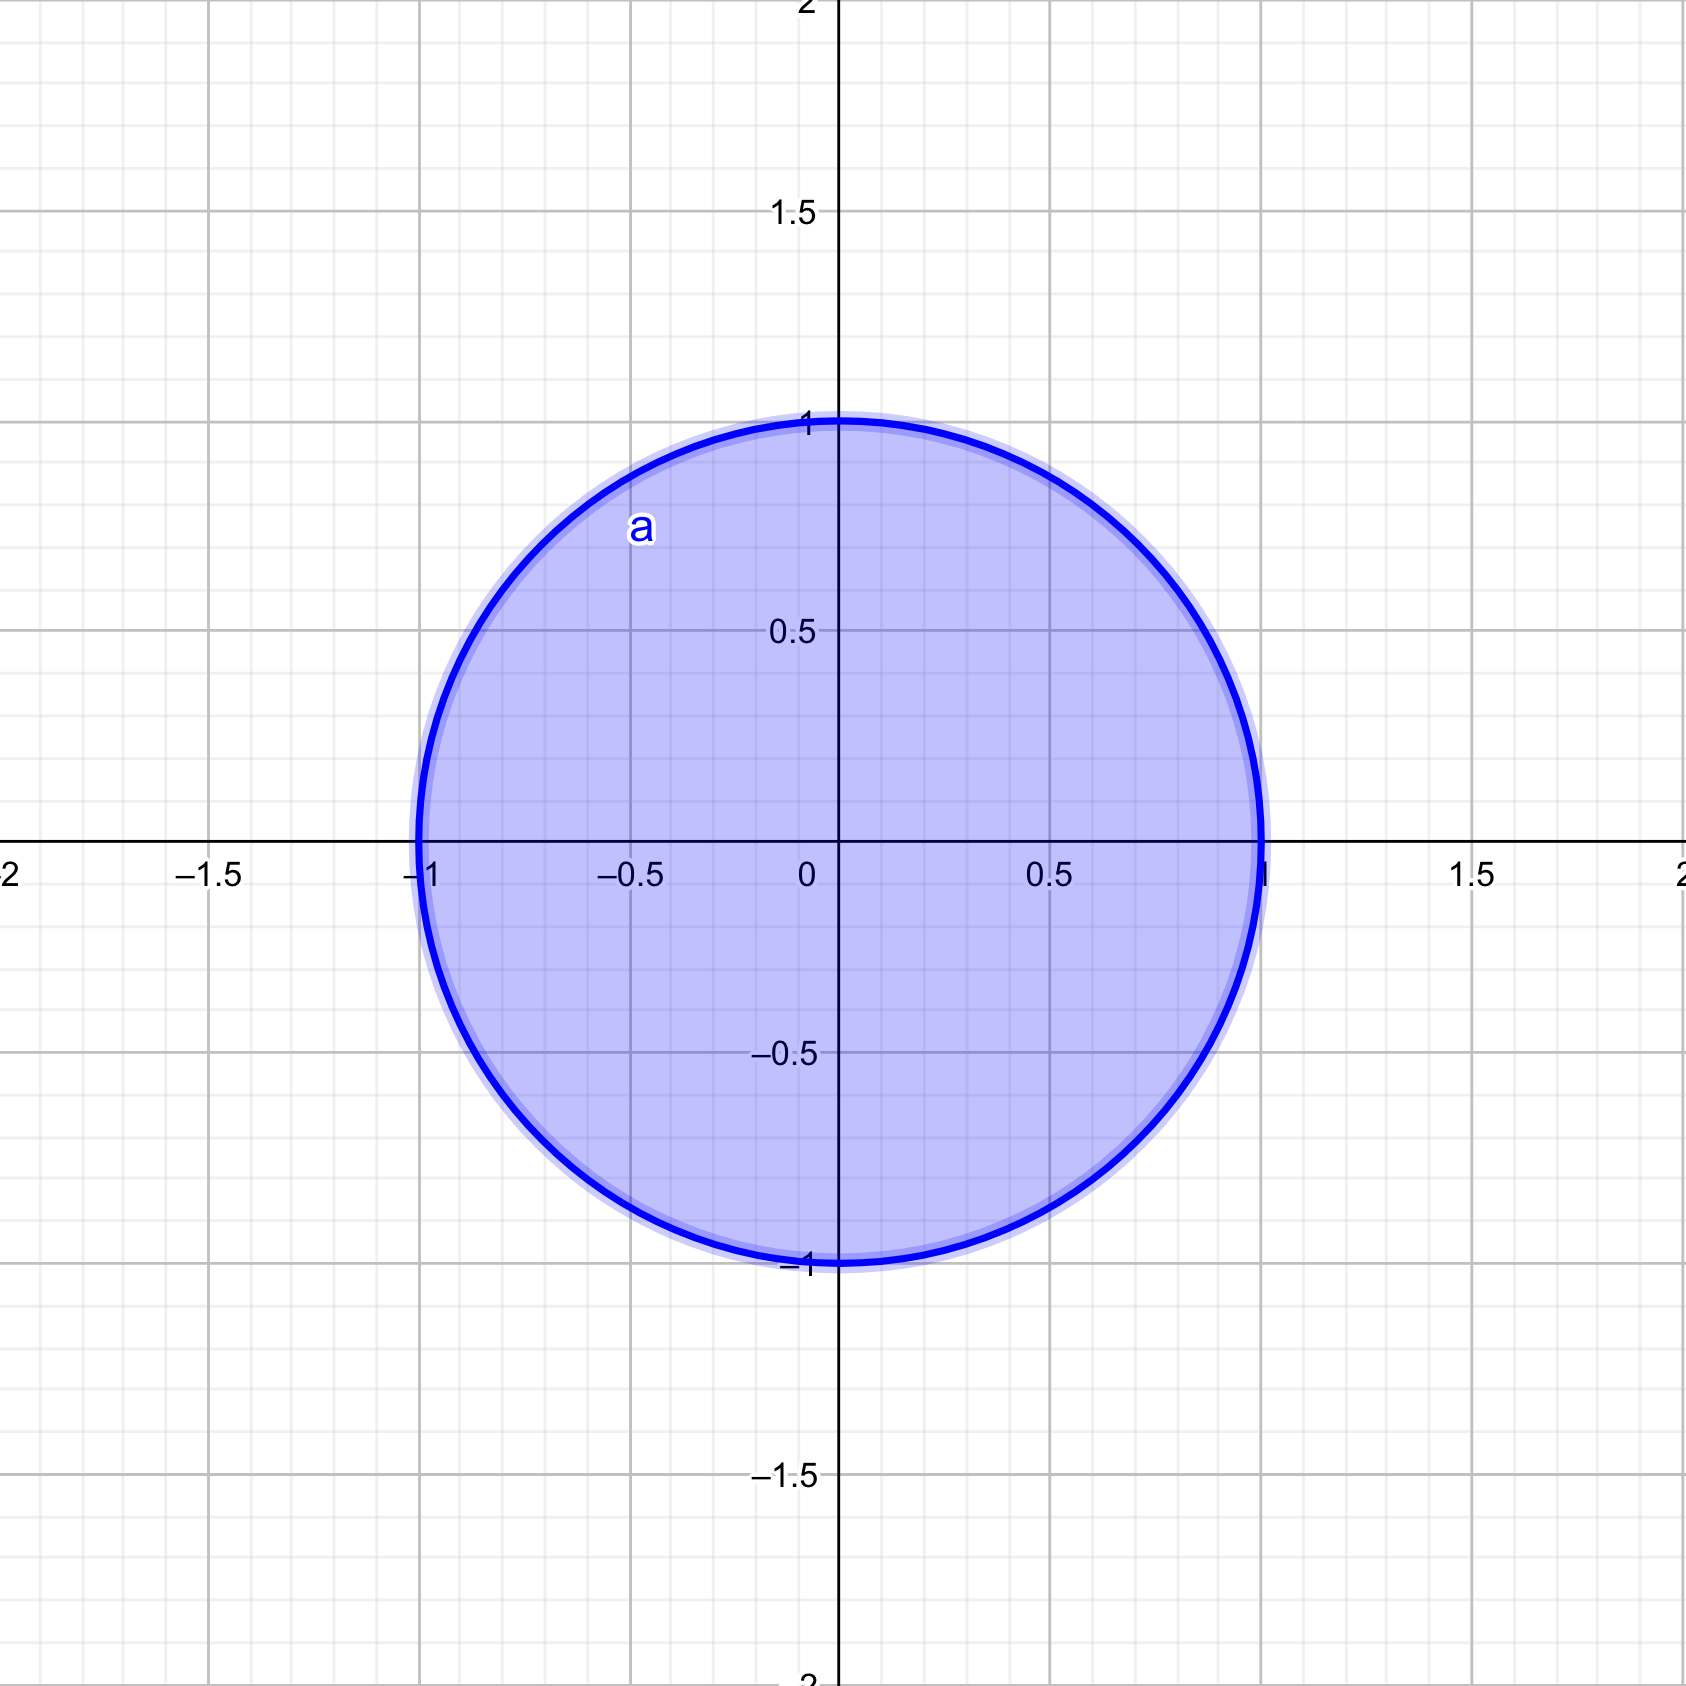
\includegraphics[width=6cm, height=6cm]{Circle1a1.png}\caption{}
            \end{figure}
            \begin{figure}[H]
                \centering
                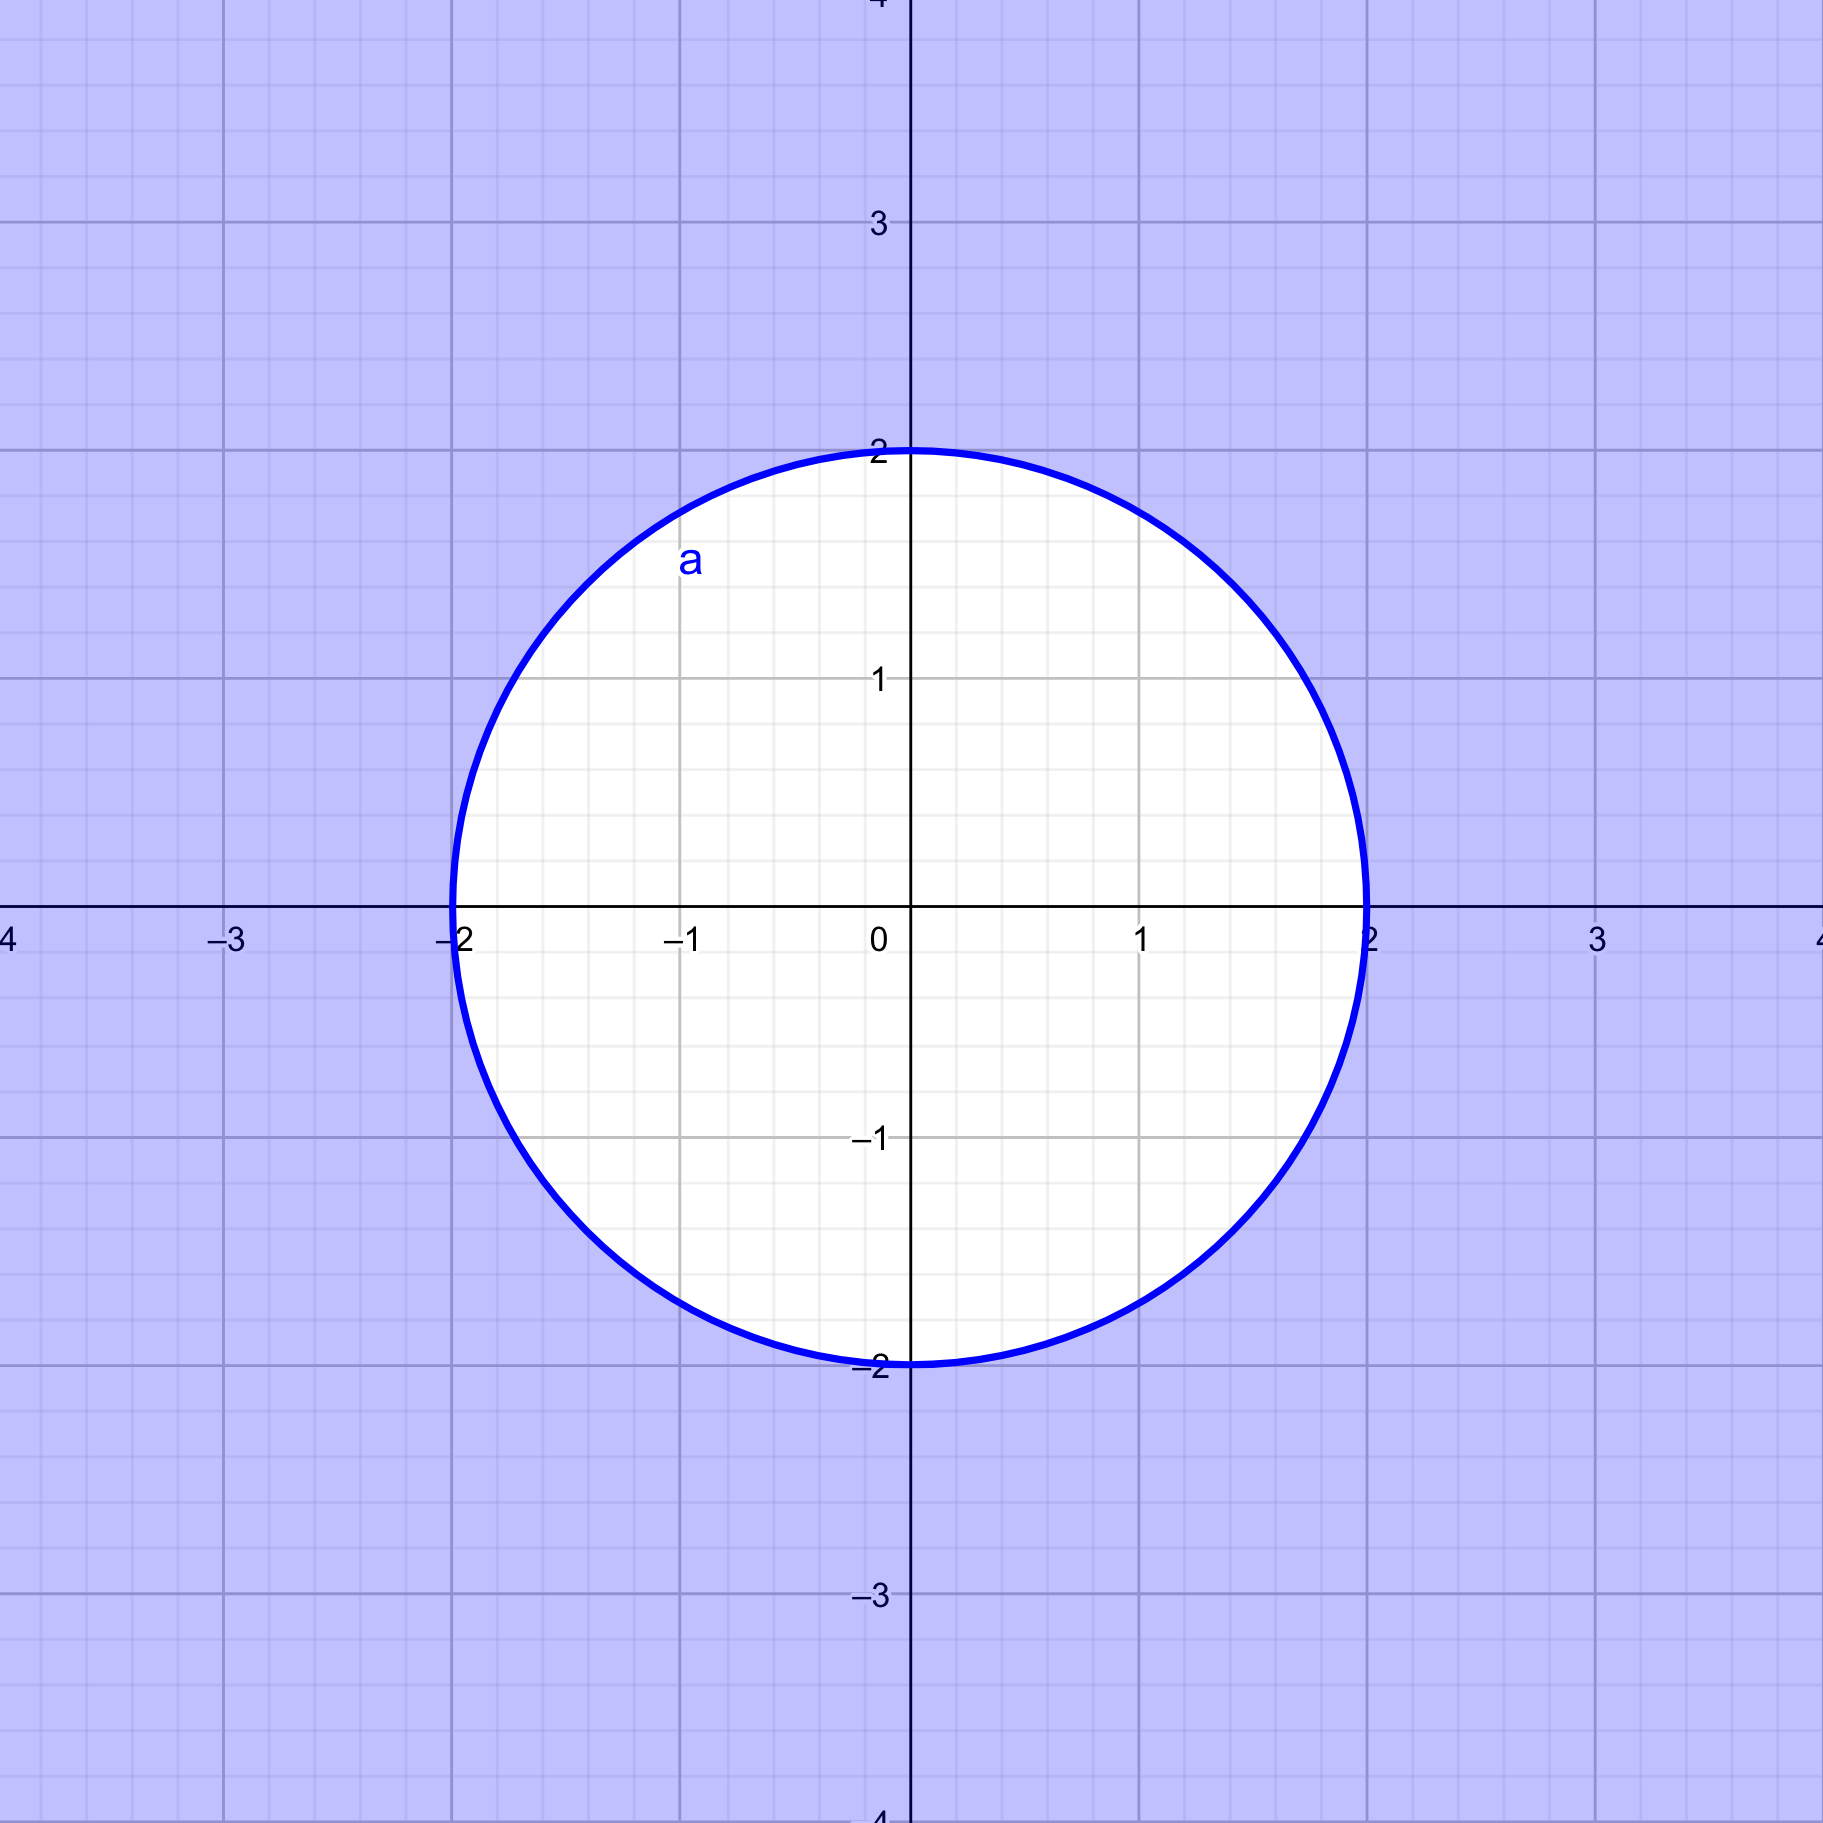
\includegraphics[width=6cm, height=6cm]{Circle1a2.png}\caption{}
            \end{figure}
            \begin{figure}[H]
                \centering
                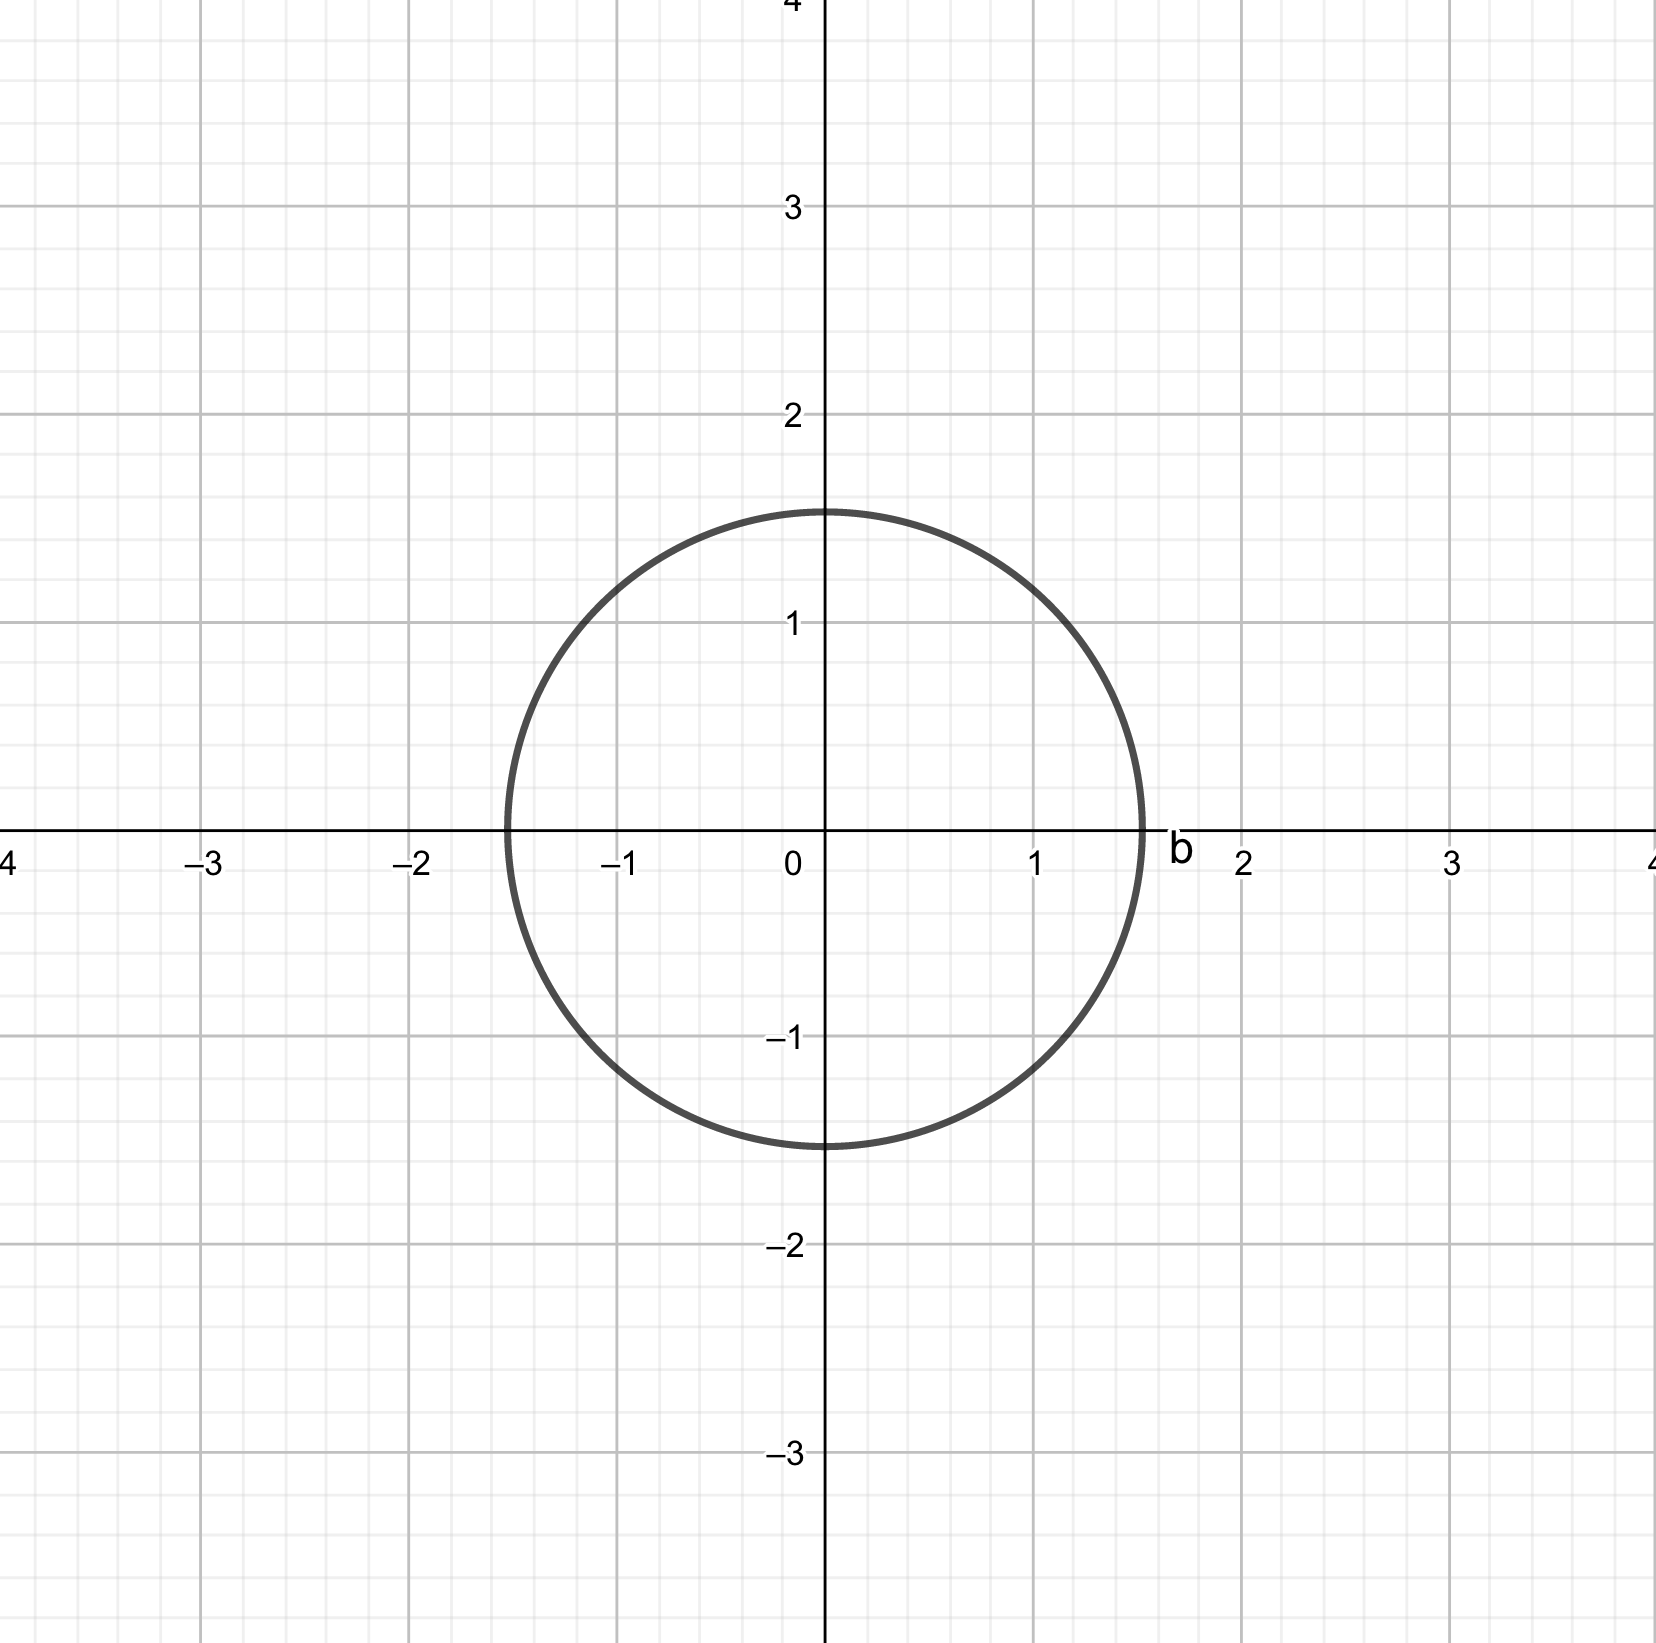
\includegraphics[width=6cm, height=6cm]{Circle1a3.png}\caption{Con \(z_0=0.2\)}
            \end{figure}
            \begin{figure}[H]
                \centering
                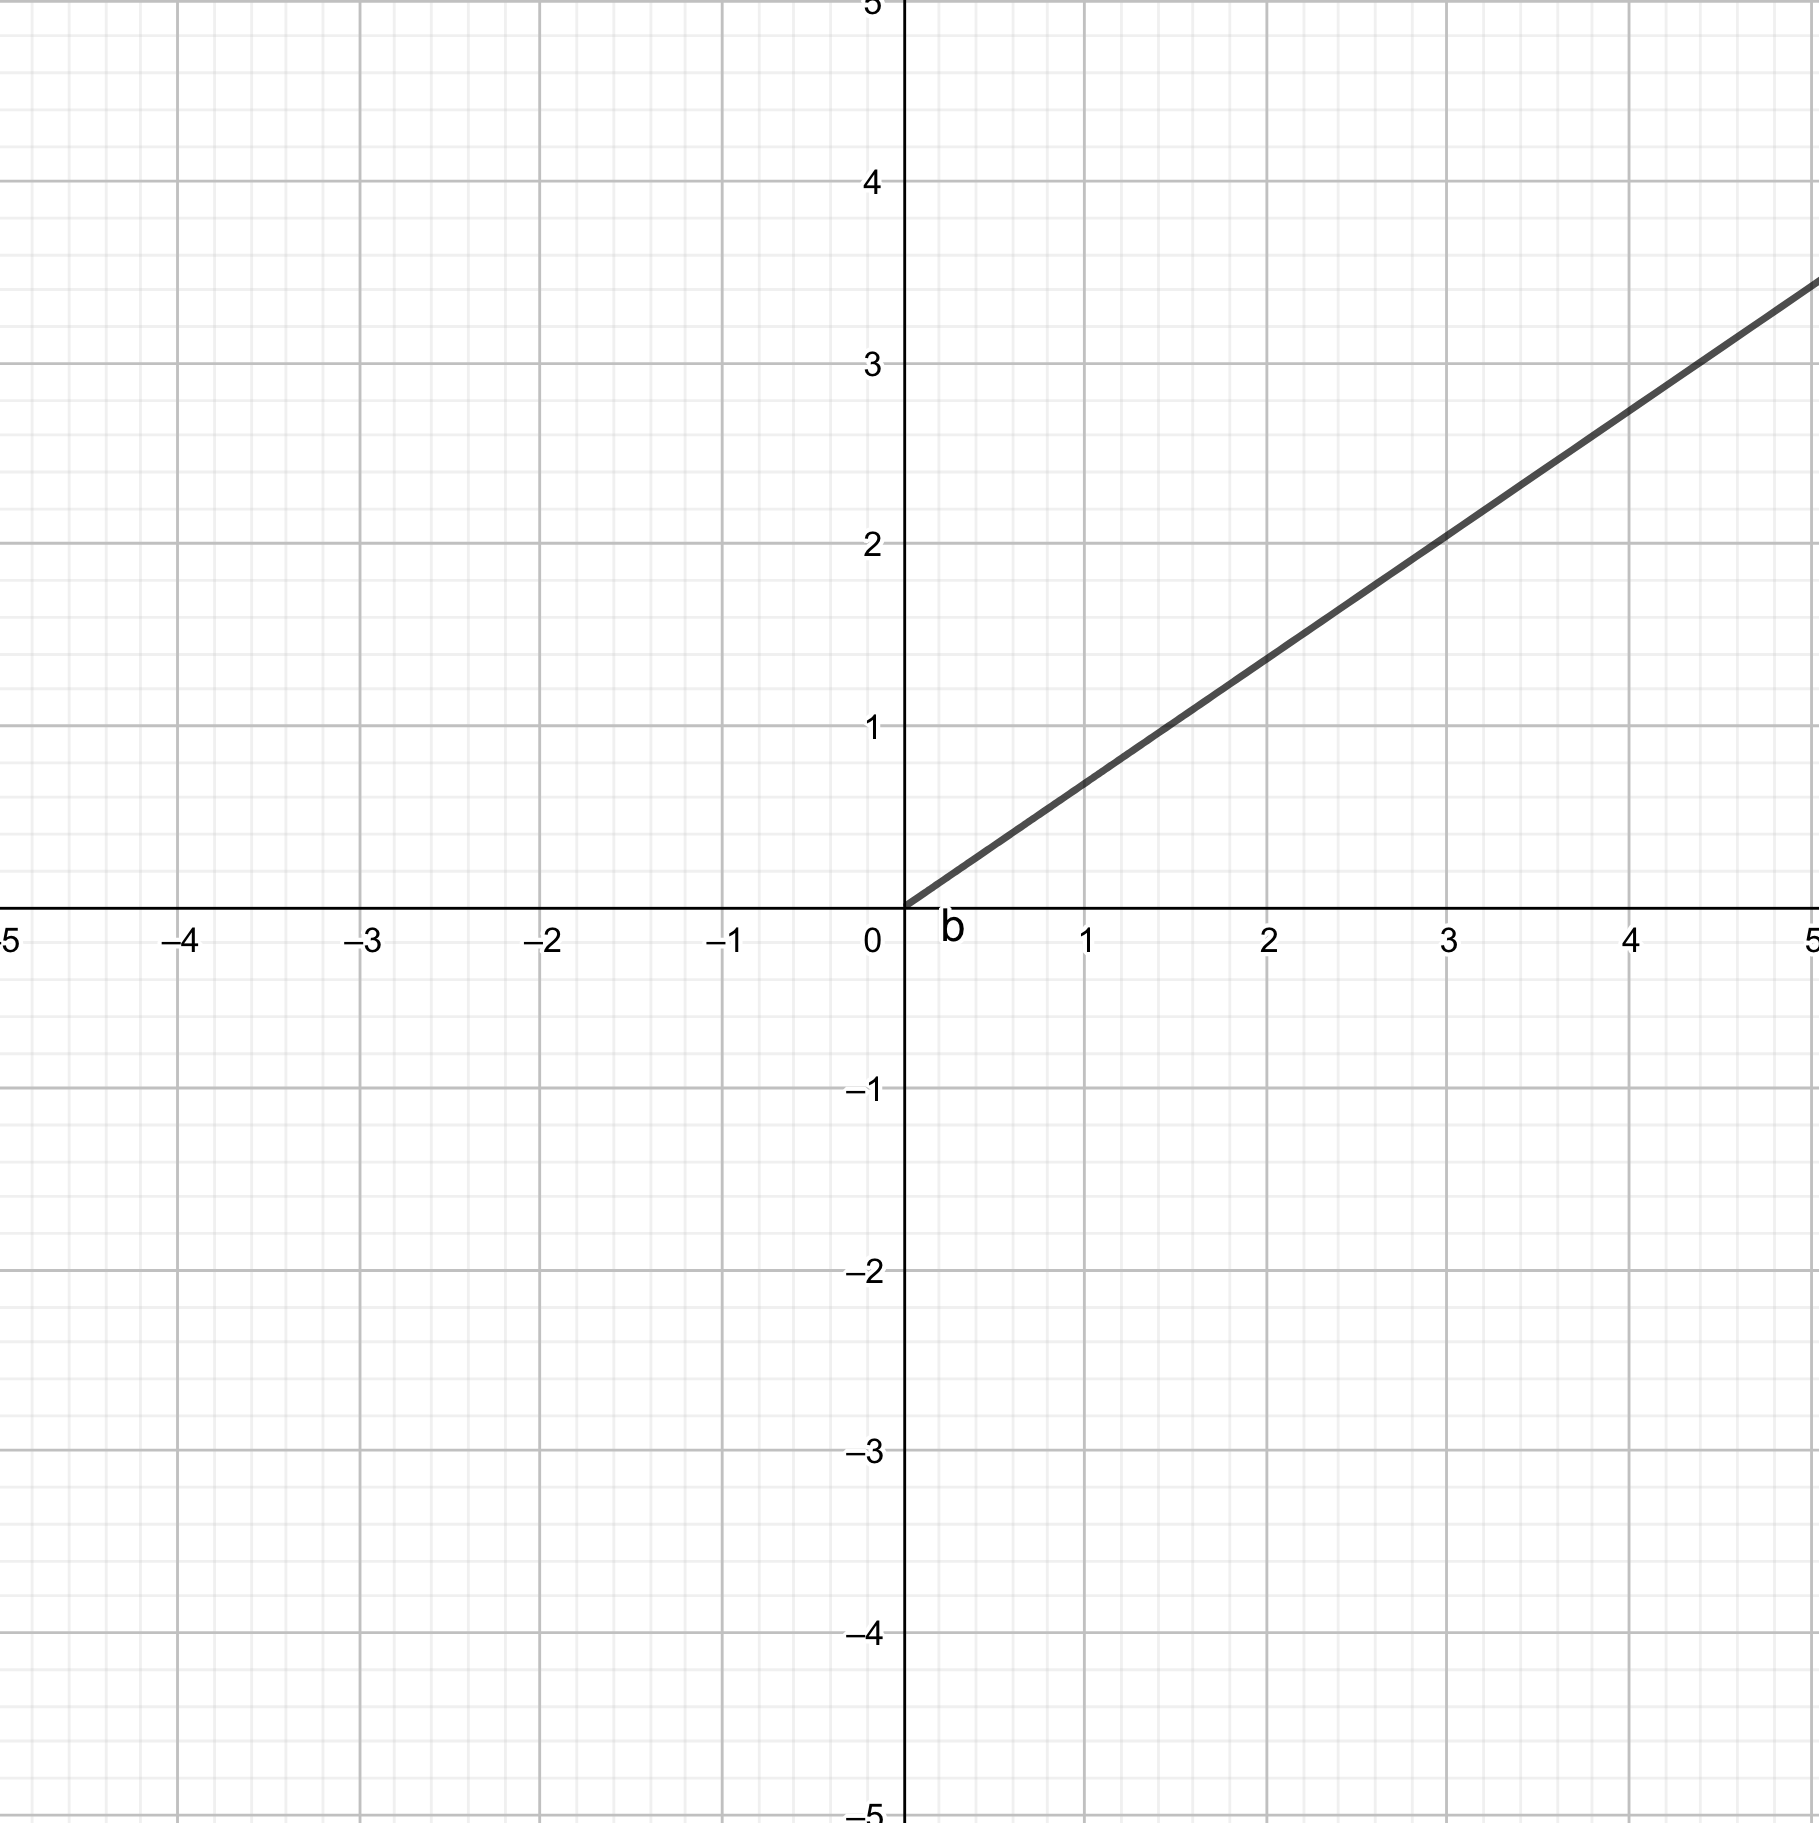
\includegraphics[width=6cm, height=6cm]{Line1a4.png}\caption{Con \(\theta=0.6\)}
            \end{figure}
        \item Sea \(f:\set{C}\rightarrow\set{S}^2\) la proyección estereográfica, y \(\rho:\set{S}^2\rightarrow\set{S}^2\) la rotación en \(\pi\) radianes respecto el eje \(x\). Se pide que \(\rho\circ f=f\circ\frac1z\). Se recuerdan las matrices de rotación, y se representa \(\rho\) como una:
              \[\rho=\begin{bmatrix}
                      1 & 0         & 0          \\
                      0 & \cos(\pi) & -\sin(\pi) \\
                      0 & \sin(\pi) & \cos(\pi)
                  \end{bmatrix}=\begin{bmatrix}
                      1 & 0  & 0  \\
                      0 & -1 & 0  \\
                      0 & 0  & -1
                  \end{bmatrix}\]
              Ahora, es claro que la rotación mapea \((x,y,z)\) a \((x,-y,-z)\). Sea \(z\in\set{C}\), se escribe como \(z=x+iy\), luego \(z\mapsto\frac{x-iy}{x^2+y^2}\), se aplica \(f\) y se llega a lo siguiente:
              \begin{equation*}
                  z\mapsto\paren{\frac{\frac{2x}{x^2+y^2}}{1+\paren{\frac{x}{x^2+y^2}}^2+\paren{\frac{-y}{x^2+y^2}}^2},\frac{\frac{-2y}{x^2+y^2}}{1+\paren{\frac{x}{x^2+y^2}}^2+\paren{\frac{-y}{x^2+y^2}}^2},\frac{-1+\paren{\frac{x}{x^2+y^2}}^2+\paren{\frac{-y}{x^2+y^2}}^2}{1+\paren{\frac{x}{x^2+y^2}}^2+\paren{\frac{-y}{x^2+y^2}}^2}}
              \end{equation*}
              Esto se puede desarrollar un poco y se llega a:
              \begin{equation*}
                  \paren{\frac{2x}{1+x^2+y^2},\frac{-2y}{1+x^2+y^2},\frac{1-x^2-y^2}{1+x^2+y^2}}
              \end{equation*}
              Con lo que claramente \(\rho\circ f=f\circ\frac1z\)
    \end{enumerate}
\end{sol}

\begin{prob}
    Encuentre mapeos conformes entre las siguientes regiones:
    \begin{enumerate}[label=(\alph*)]
        \item \(\{z\in\set{C}:\abs{z}<1\}\) y \(\{z\in\set{C}:\abs{z}>1\}\).
        \item \(\{r\exp(i\theta)\in\set{C}:\theta\in(0,\frac\pi{n}),r\in\set{R}\}\) y \(\set{C}\), con \(n\in\set{N}\setminus\{0\}\).
        \item \(\{z\in\set{C}:\abs{z}>1\}\) y \(\{z\in\set{C}:\Im(z)>0\}\).
        \item \(\{z\in\set{C}:\Re(z)>0\}\) y \(\{z\in\set{C}:\Im(z)\in(-\frac\pi2,\frac\pi2)\}\).
        \item \(\{z\in\set{C}:\abs{z}>1\}\) y \(\{z\in\set{C}:\Im(z)\in(a,b)\}\)
    \end{enumerate}
\end{prob}

\begin{sol}
    \begin{enumerate}
        \item Se recuerda que la inversión es un mapeo conforme, y que mapea las regiones pedidas.
        \item Se recuerda que las funciones analíticas son mapeos conformes, se toma \(f(x)=x^{n+1}\) se nota que cumple lo pedido.
        \item Se ven las proyecciones de ambas regiones en la esfera y se nota que ambas son hemisferios, por lo que una rotación en la esfera cumple lo pedido.
        \item Se nota que \(z\mapsto\exp(z)\) mapea \(\{z\in\set{C}:\Im(z)\in(-\frac\pi2,\frac\pi2)\}\) a \(\{z\in\set{C}:\Re(z)>0\}\). Y \(\exp(z)\) es analítica, por lo que se tiene el mapeo conforme.
        \item Usando los mapeos anteriores (los cuales son todos biyectivos excepto \(x^{n+1}\)) y el mapeo lineal \(f\) de \(\{z\in\set{C}:\Im(z)\in(a,b)\}\) a \(\{z\in\set{C}:\Im(z)\in(-\frac\pi2,\frac\pi2)\}\), se hace la siguiente cadena de mapeos conformes, se usa \(f\), luego \(\exp(z)\), se rota en la esfera para llegar a \(\{z\in\set{C}:\abs{z}>1\}\) y se invierte.
    \end{enumerate}
\end{sol}

\begin{prob}
    Sea \(h:[0,1]\rightarrow\set{C}\) continua y se define en \(\set{C}\setminus[0,1]\) la función
    \[H(z)=\int_0^1\frac{h(t)}{t-z}\d{t}.\]
    Demuestre que \(H\) es analítica y calcule por definición su derivada.
\end{prob}

\begin{sol}
    Se nota que si para cada \(z_0\in\set{C}\setminus[0,1]\), se tiene que
    \begin{equation}
        \lim_{z\rightarrow z_0}\abs{\frac{H(z)-H(z_0)}{z-z_0}-\int_0^1\frac{h(t)}{(t-z_0)^2}\d{t}}=0\label{limHz}
    \end{equation}
    Entonces, \(H(z)\) es analítica. Luego, se nota que dado \(z_0\in\set{C}\setminus[0,1]\), se tiene \(0<\inf_{t\in[0,1]}\abs{t-z_0}=\gamma\). Dado esto, se tiene que si \(\abs{z-z_0}<\gamma/2\) entonces \(\abs{z-t}>\gamma/2\) para \(t\in[0,1]\). Ahora desarrollando la siguiente expresión:
    \begin{align*}
        \abs{\frac{H(z)-H(z_0)}{z-z_0}-\int_0^1\frac{h(t)}{(t-z_0)^2}\d{t}} & =\abs{\int_0^1\frac{h(t)(t-z-t+z_0)}{(z-z_0)(t-z)(t-z_0)}-\int_0^1\frac{h(t)}{(t-z_0)^2}\d{t}} \\
                                                                            & =\abs{\int_0^1\frac{h(t)}{t-z_0}\cdot\paren{\frac1{t-z}-\frac1{t-z_0}}\d{t}}                   \\
                                                                            & =\abs{\int_0^1\frac{h(t)}{t-z_0}\cdot\paren{\frac{z_0-z}{(t-z)(t-z_0)}}\d{t}}                  \\
                                                                            & \leq\int_0^1\abs{\frac{h(t)}{(t-z_0)^2}\cdot\frac1{t-z}\cdot(z-z_0)}\d{t}                      \\
                                                                            & \leq\int_0^1\abs{\frac{h(t)}{(t-z_0)^2}\cdot\frac2\gamma}\d{t}\cdot\abs{z-z_0}
    \end{align*}
    Con lo que claramente el límite en \eqref{limHz} es cero.
\end{sol}

\begin{prob}
    Considere un dominio \(D\) y \(f:D\rightarrow\set{C}\) analítica. Se define \(D^*=\{\overline{z}:z\in D\}\) y \(g(z)=\overline{f(\overline{z})}\) para \(z\in D^*\). Demuestre que \(g\) analítica y calcule su derivada.
\end{prob}

\begin{sol}
    Sea \(g(x,y)=u_2(x,y)+iv_2(x,y)\) con \(f(x,y)=u_1(x,y)+iv_1(x,y)\), entonces se tiene que \(u_2(x,y)=u_1(x,-y)\) y \(v_2(x,y)=-v_1(x,-y)\). Ahora, se calculan las derivas parciales de \(u_2\) y \(v_2\):
    \begin{align*}
        \frac{\partial u_2}{\partial x}(x,y) & =\frac{\partial u_1}{\partial x}(x,-y)          & \frac{\partial v_2}{\partial x}(x,y) & =-\frac{\partial v_1}{\partial x}(x,-y)          \\
                                             & =\frac{\partial v_1}{\partial y}(x,-y)          &                                      & =-\paren{-\frac{\partial u_1}{\partial y}(x,-y)} \\
                                             & =-\paren{-\frac{\partial v_2}{\partial y}(x,y)} &                                      & =-\frac{\partial u_2}{\partial y}(x,y)           \\
                                             & =-\frac{\partial v_2}{\partial y}(x,y)          &                                      &
    \end{align*}
    Con esto, se ve que \(g\) cumple las condiciones de Cauchy-Riemann, por lo que es analítica.
\end{sol}

\begin{prob}
    Considere \(f=u+iv\) analítica. Demuestre que
    \begin{enumerate}[label=(\alph*)]
        \item \(\abs{\nabla u}=\abs{\nabla v}=\abs{f'}\)
        \item \(\angled{\nabla u,\nabla v}=0\)
    \end{enumerate}
\end{prob}

\begin{sol}
    \begin{enumerate}
        \item Se recuerda que el siguiente limite existe si no depende del camino tomado:
              \[\lim_{z\rightarrow z_0}\frac{f(z)-f(z_0)}{z-z_0}\]
              Por lo que \(u'=\frac{\partial u}{\partial x}=\frac{\partial u}{\partial y}\), análogamente para \(v\). Con esto y usando la condición de Cauchy-Riemann, se ve la siguiente igualdad:
              \[\paren{\frac{\partial u}{\partial x}}^2+\paren{\frac{\partial u}{\partial y}}^2=\paren{\frac{\partial v}{\partial y}}^2+\paren{\frac{\partial v}{\partial x}}^2=\paren{u'}^2+\paren{v'}^2\]
              Con lo anterior es claro que \(\abs{\nabla u}=\abs{\nabla v}=\abs{f'}\).
        \item Al calcular el gradiente de \(u\) y de \(v\) se ve lo siguiente:
              \begin{align*}
                  \angled{\nabla u,\nabla v} & = \frac{\partial u}{\partial x}\frac{\partial v}{\partial x}+\frac{\partial u}{\partial y}\frac{\partial v}{\partial y} \\
                                             & =\frac{\partial u}{\partial x}\frac{\partial v}{\partial x}-\frac{\partial u}{\partial x}\frac{\partial v}{\partial x}  \\
                                             & =0
              \end{align*}
              Con lo que se tiene lo pedido.
    \end{enumerate}
\end{sol}

\begin{prob}
    Sea \(f:D\rightarrow\set{C}\) inyectiva y analítica. Demuestre que
    \[\text{Area}(f(D))=\iint_D\abs{f'(z)}^2\d{x}\d{y}\]
\end{prob}

\begin{sol}
    Sea \((x,y)\mapsto(u(x,y),v(x,y))\) un cambio de coordenadas, este esta bien definido en \(D\) ya que \(f\) es inyectiva y analítica. Luego, se calcula la inversa del Jacobiano:
    \[J^{-1}=\begin{bmatrix}
            \frac{\partial u}{\partial x} & \frac{\partial u}{\partial y} \\
            \frac{\partial v}{\partial x} & \frac{\partial v}{\partial y}
        \end{bmatrix}\]
    Con esto y la condición de Cauchy-Riemann se nota que \(\ds\abs{J^{-1}}=\paren{\frac{\partial u}{\partial x}}^2+\paren{\frac{\partial u}{\partial y}}^2\), lo cual por la pregunta anterior es \(\abs{f'}^2\). Se aplica la transformación a la siguiente integral:
    \[\iint_D\abs{f'(z)}^2\d{A}\]
    Con lo que queda:
    \[\iint_D\abs{f'(z)}^2\d{A}=\iint_{f(D)}1\d{A}=\text{Area}(f(D))\]
\end{sol}

\begin{prob}
    Decimos que una función \(f:D\subset\set{C}\rightarrow\set{C}\) es armónica si \(\Re(f)\) e \(\Im(f)\) son armónicas. Demuestre que si  \(h\) y \(zh\) son armónicas, entonces \(h\) es analítica.
\end{prob}

\begin{sol}
    Se recuerda que si una función \(f\) es armónica entonces \(\Delta f=0\), o equivalentemente, \(\ds\sum_{i=1}^n\frac{\partial^2f}{\partial x_i^2}=0\). Sea \(h=u+iv\) una función armónica tal que \(zh\) también lo sea, entonces \(\frac{\partial^2 u}{\partial x^2}+\frac{\partial^2 u}{\partial y^2}=0\) y \(\frac{\partial^2 v}{\partial x^2}+\frac{\partial^2 v}{\partial y^2}=0\), además se tiene lo siguiente:
    \begin{align*}
        0 & =\frac{\partial^2 (ux-vy)}{\partial x^2}+\frac{\partial^2 (ux-vy)}{\partial y^2}                                                                                                                           \\
          & =x\frac{\partial^2 u}{\partial x^2}+2\frac{\partial u}{\partial x}-y\frac{\partial^2 v}{\partial x^2}-y\frac{\partial^2 v}{\partial y^2}-2\frac{\partial v}{\partial y}+x\frac{\partial^2 u}{\partial y^2} \\
          & =2\paren{\frac{\partial u}{\partial x}-\frac{\partial v}{\partial y}}
    \end{align*}
    Similarmente:
    \begin{align*}
        0 & =\frac{\partial^2 (uy+vx)}{\partial x^2}+\frac{\partial^2 (uy+vx)}{\partial y^2}                                                                                                                           \\
          & =y\frac{\partial^2 u}{\partial x^2}+2\frac{\partial v}{\partial x}+x\frac{\partial^2 v}{\partial x^2}+y\frac{\partial^2 u}{\partial y^2}+2\frac{\partial u}{\partial y}+x\frac{\partial^2 v}{\partial y^2} \\
          & =2\paren{\frac{\partial v}{\partial x}+\frac{\partial u}{\partial y}}
    \end{align*}
    Con ambas se tiene que \(\frac{\partial u}{\partial x}=\frac{\partial v}{\partial y}\) y \(\frac{\partial v}{\partial x}=-\frac{\partial u}{\partial y}\), las cuales son las condiciones de Cauchy-Riemann. Con esto se tiene que \(h\) es analítica.
\end{sol}

\end{document}
